\documentclass{llncs}
%
\usepackage{url}
\RequirePackage[hyphenbreaks]{breakurl} % allow hyphenation in URLs
\usepackage{amsmath} % use equations
\usepackage{graphicx} % allow PNGs as graphics
\usepackage{subfigure}
\usepackage{float}
\RequirePackage[utf8]{inputenc} % support Umlauts and special characters
\usepackage{microtype} % use space more efficiently and hyphenate smarter: all in all looks a lot sexier
\usepackage{listings} % allow source code environments
% Define a listing style for FLUX code
\lstdefinestyle{flux} {
  frame=L,
  xleftmargin=\parindent,
  basicstyle=\footnotesize\ttfamily,
  breakatwhitespace=true,
  numbers=left,
  escapechar=\%,
  numberstyle=\tiny,
  numberblanklines=false,
  captionpos=b,
  emph={perform, poss, state\_update, main\_loop, init},
  emphstyle=\textbf,
}
%
\title{Research Lab "Multi-Agent Programming Contest 2014"}
\subtitle{Final Report}
%\titlerunning{logprog}
\author{Artur Daudrich \and Sergey Dedukh \and Maunuel Mittler \and Michael Ruster \and Michael Sewell \and Yuan Sun}
\institute{University of Koblenz-Landau, Koblenz Campus}
%\tocauthor{ }
%
\begin{document}
\maketitle

\section{Implementation Details}
\subsection{BDI in AS(L) and Jason}

BDI model is one of the most used architectures for cognitive agents. AgentSpeak(L) is one of the most popular agent-oriented programming languages based on BDI model.

AgentSpeak(L) is a programming language based on a restricted first-order language with events and actions \cite{anand_AgentSpeak_1996}. What was written in AgentSpeak(L) decides the behaviour of an agent, such like the agent's interactions with the environment. In other words, we can design the beliefs, desires, and intentions of the agent by writing these notions in AgentSpeak(L) instead of representing them as model formulas explicitly.

Beliefs are the current states of the agent which are not immutable but updated when the environment changes or some events that can affect agents' beliefs are triggered; states which the agent wants to bring about based on its external or internal stimuli can be viewed as desires; and the adoption of programs to satisfy such stimuli can be viewed as intentions\cite{anand_AgentSpeak_1996}. 

Jason is a Java-based platform that can interpret for an extended version of AgentSpeak and it makes AgentSpeak language practically suitable for multi-agent systems, therefore we implement Jason for this multi-agent system programming. 

An AgentSpeak agent is defined by a set of beliefs giving the initial state of the agent’s belief base, which is a set of ground (first-order) atomic formula, and a set of plans which form its plan library\cite{rafael_BDIAgent_2005}. In our multi-agent programming, 34 kinds of basic beliefs are stored. These beliefs describe basic current states of each agent such as the name of an agent, the energy, the role and so on. These beliefs are not immutable and can be used in writing plans and goals. 

Desires in BDI model are always treated as goals. A goal of AgentSpeak has two types: achievement goal and test goal. When the associated atomic formula is true, and the agent wants to achieve a state of the world, it is stated as an achievement goal with being formed by an atomic formula prefixed with the ‘!’. On the other hand, A test goal which is prefixed with the ‘?’ operatorstates that the agent wants to test whether the associated atomic formula is (or can be unified with) one of its beliefs \cite{rafael_BDIAgent_2005}. We mostly implement achievement goals in our program, because achieving some states are always wanted. For example, "!doParry." is an achievement goal that will execute the "parry" action when some events are triggered. Although achievement goals occupy about 99 percent of the goals, we still implement three test goals such as "?maxRange(MaxRange)" which checks the current range is maximum or not when finding the best zone for agents. All of these three test goals are implemented in zone building, and all the remaining goals are achievement goals.

As known, only goals' existing is not enough, we need trigger events to achieve the goals in a plan. Similar with goals, an event also has two types: internal trigger event and external trigger event. An event is internal when a sub-goal needs to be achieved and an external event is generated from belief updates as a result of perceiving the environment. We have 88 events in total in our program and two of them are presented as follow:
\begin{figure}
\centering%
\begin{minipage}[!htbp]{\linewidth}
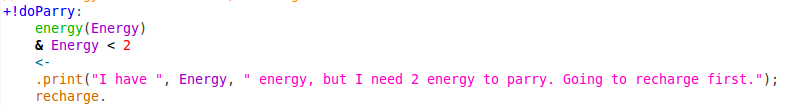
\includegraphics[width=5.0in]{images/BDI_trigger_event_Inter}
\caption{Internal Trigger Event}
\label{fig:latticen}
\end{minipage}
\begin{minipage}[!htbp]{\linewidth}
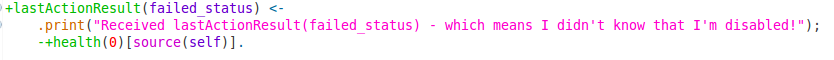
\includegraphics[width=5.0in]{images/BDI_trigger_event_Exter}
\caption{External Trigger Event}
\label{fig:baselinex}
\end{minipage}
\end{figure}

In Fig.1, we see the internal trigger event "+!doParry" which is for achieving the goal "doParry", on the other hand, in Fig.2 the trigger event "+lastActionResult(failed\underline{ }status)" is external which means when the belief "last action result is failed\underline{ }status" has been added, it will execute what is shown in the body of this plan.

With beliefs, trigger events and goals, we can make plans for each agent. An AgentSpeak plan consists of a head which is formed from a triggering event, a conjunction of belief literals representing a context,and a body which is a sequence of basic actions or goals that the agent has to achieve when the plan is triggered\cite{rafael_BDIAgent_2005}. In our program, there are 184 plans in total. 101 of them have the head of internal trigger events as well as 83 plans are with the head of external trigger events. The plans with internal trigger events are 18 more than those with external events, that means when plans are made, we add or delete goals which generated from the agent’s own execution of a plan much more than adding or deleting beliefs based on perception. 

Different plans can ensure to complete different tasks which are required to be done by several kinds of agents. In this multi-agent system, several actions are already defined before starting this program. What required to do is to make good plans to let different agents implement these actions well so that good points can be acquired. For example, 6 out of 28 agents are allowed to execute the action "attacking". When we try to make plans for the agents who can attack, a variety of situations should be considered of; like when the enemy stands on the neighbour node of our agents, or when our agents don't find any enemies nearby, laying different plans is necessary. Of course, the allocation of plans' quantity can not be the same for executing different actions, because strategies for executing various actions differ under different circumstances. The arrangement for the amount of plans of different actions is presented in Fig.4.
\begin{figure}[H]
\centering
\begin{minipage}[!htbp]{\linewidth}
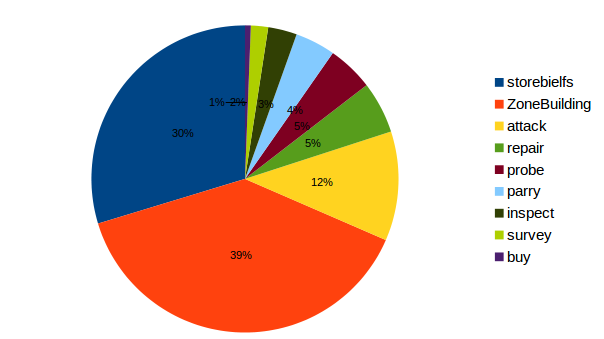
\includegraphics[width=5.0in]{images/BDI_plan_allocation}
\caption{allocation for number of plans}
\label{fig:plan_allocation}
\end{minipage}
\end{figure}

As we can see, building zones occupies 39 percent of the plans and the second largest part is contributed by the basic beliefs storing. However, all the plans for storing basic beliefs are with external trigger events meanwhile they are very fundamental. For instants, "+health(Numeral)[source(percept)] $<- \ -+$health(Numeral)[source(self)]." is just to store the health updating every step. Therefore, basic beliefs storing can be ignored in this comparison. Obviously, zone building uses more plans than others. It is easy to know that building a zone is more complex than other action executing. Zone building will be affected by the maps given in the contest, the position where the agents of other teams occupy and many other situations as well. Additionally, building a good zone will get a lot of scores so more strategies focusing on zone building is reasonable. Compared with zone building, the plan for the action "buy" is easy. When the specified agent "Saboteur" don't see any enemy agents nearby, it will "buy" more "health" and "visibility range".Action "attack" uses a little more plans than other remaining actions since the strategy is designed offensively. Making agents from other teams disabled is our purpose, moreover the action "attack" should be executed rapidly and effectively. Consequently, in contrast, more plans are adopted by the action "attack".

Intentions are particular courses of actions to which an agent has committed in order to handle certain events. Each intention is a stack of partially instantiated plans\cite{rafael_Javabased_2007}. The execution of plans may be started off by their trigger events. As mentioned above, trigger events can be external when coming from the perception of changing environment, or internal when generated from the sub-goals. We know that, applicable plans were chosen and putted into the intention stack. If the chosen plan is for an internal event, it will be pushed on top of that intention. Otherwise, if the chosen plan has a head with an external trigger event, it will create a new intention and store in the intention stack. The allocations of this two types of plans are different for various agents. According to a rough statistic, we can find the differences in the following figures.
\begin{figure}
\centering
\begin{minipage}[!htbp]{\linewidth}
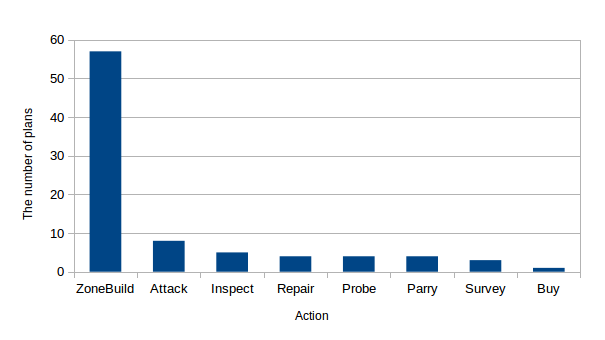
\includegraphics[width=5.0in]{images/BDI_plan_distribution_action}
\caption{plan distribution for actions}
\label{fig:plan_allocation}
\end{minipage}
\end{figure}
\begin{figure}
\centering
\begin{minipage}[!htbp]{\linewidth}
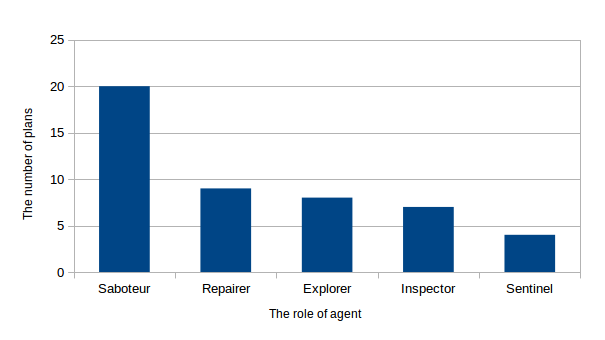
\includegraphics[width=5.0in]{images/BDI_plan_distribution_role}
\caption{plan distribution for agents}
\label{fig:baselinex}
\end{minipage}
\end{figure}
 
In figure 4, we can see that all plans used by storing basic beliefs are with external trigger events as mentioned above. Besides that, only zone building and execution of action "attack" adopt plans with external trigger events. The other remaining actions use few plans with external trigger events. In general, internal trigger events are more often used in plans. After calculating, about 41 percent of plans for zone building are for external trigger events but 23 percent of plans for execution of "attack" are for external trigger events. So more zone building plans are triggered by the perception of the agent’s environment than that for "attack". In this program, plans with internal trigger events which generated from the agent’s own execution of a plan are adopted widely. Therefore, the execution of the previous plan makes more sense to the current plan of agents than the perception of the environment's impact.

Agents in this multi-agent system are divided into five classes by their roles---explorer, saboteur, repairer, sentinel, and inspector. They have various tasks to do to achieve points in the contest, moreover, the number of plans adopted by them are definitely different which can be seen in figure 5. It is notable that what figure 5 presenting has removed the plans which available to be used by all kinds of agents such as going to another node, and presenting particular plans that only used by their relevant agents. Similar as the plan distribution for different actions, most plans are for internal triggered events. Just "saboteur" which the only role of agents can do action "attack" use the plans with external trigger events and this kind of plans do not occupy a big part.
Furthermore, saboteurs using most plans is in accordance with our offensive strategy. Explorers, repairers and inspectors use about the same amount of plans, however, few plans are for sentinels. This is reasonable in view of there is not any actions only available for sentinels.

Beliefs, desires and intentions are introduced above, but many agentspeak languages contain all these three. One of the reasons to choose Jason as programming language is that Jason can either provide a library of essential internal actions, or be straightforward extensible by user-defined internal actions, which are programmed in Java\cite{rafael_Javabased_2007}. Implementing internal actions provides the means for programmers to do important things for BDI-inspired programming, such as checking and dropping the agent’s own
desires/intentions\cite{rafael_overviewjason_2006}. Besides the original internal actions like ".print" or ".send", 32 internal actions defined by our own are programmed in Java. Most of these internal actions are devoted to control the map, such as calculating the distance between two agents or searching the nearest position to the current Vertex and so on. These internal actions run internally by the agent resulting in saving the commuting time.

Although Jason is a kind of new language for our team members, it is considered as the best agent speak language chosen for this multi-agent system after we trying to learning it. In our program, BDI model is clearly described, meanwhile beliefs, desires and intentions are arranged reasonably. In addition, the features of jason such as user-defined internal actions are great used to improve communication process in our program. All our effort contributes in acquiring the second place in this contest. However, not familiar with Jason also makes some problems, some functions are not implemented completely, or some strategy is not the most reasonable. There is still room for improvement and many things need to be perfect.

 


\bibliographystyle{plain}
\clearpage
\bibliography{tech.bib}
\end{document}